%! TEX root = /home/hsartoris/sproj/writeup/main.tex
\graphicspath{ {resources/models/3neurEx/} {resources/models/3neurEx/weights/} } 

\chapter{Results}
\label{results}
\section{Overfitting}
\label{sec:overfitting}
\setlength{\columnsep}{20pt}
\begin{wraptable}[8]{r}{.4\textwidth}
	\captionsetup{justification=centering}
	\vspace{-20pt}
	\begin{tabular}{lr}
		b (timesteps) & 8\\
		d& 5\\
		Batch size& 32\\
		Training steps& 20000\\
		Learning rate& .0005\\
		Training samples& 18000\\
		Validation samples& 4500
	\end{tabular}
	\vspace{-5pt}
	\captionof{figure}{\linespread{1.2}\selectfont{}Training parameters for null 
		hypothesis networks}
	\label{fig:nullparams}
\end{wraptable}
As discussed in \ref{subsec:hotswap} and \ref{subsec:n-independence}, the unique 
structure of our model prevents it from overfitting to a particular generator 
topology, allowing us to create a single generator containing connections 
representative of the types of data we expect to analyze with the trained model.
We demonstrate this aspect of our architecture in two test cases: by training 
models on an empty dataset paired with one adjacency matrix throughout, and 
training with a random dataset paired with that same adjacency matrix.

\subsection{Empty Data}
\label{subsec:empty}
We ran a combined 100 training sessions of the benchmark model and our 
convolutional model, with parameters as defined in \figref{fig:nullparams}, on a 
dataset whose inputs contained only zeroes and whose target was the adjacency 
matrix in \figref{fig:2simplex+adjacency}. For both models, exactly two losses 
and corresponding outputs repeatedly occurred (\figref{fig:empty_loss}), with 
the models demonstrating a total inability to memorize the target data.

\begin{figure}[h]
	\centering
	\begin{subfigure}{.45\textwidth}
		\centering
		\begin{tabular}{cccc}
				   &  0 &  1 &  2\\\cline{2-4}
			\mc{0} & .3 & .3 & .3\\
			\mc{1} & .3 & .3 & .3\\
			\mc{2} & .3 & .3 & .3
		\end{tabular}
		\caption{loss: $0.\overline{6}$}
		\label{subfig:empty_loss0}
	\end{subfigure}
	\begin{subfigure}{.45\textwidth}
		\centering
		\begin{tabular}{llll}
			  & 0 & 1 & 2\\\cline{2-4}
			\mc{0} & 0 & 0 & 0\\
			\mc{1} & 0 & 0 & 0\\
			\mc{2} & 0 & 0 & 0
		\end{tabular}
		\caption{loss: 1.0}
		\label{subfig:empty_loss1}
	\end{subfigure}
	\caption{Predictions and losses when training on an empty dataset}
	\label{fig:empty_loss}
\end{figure}

\subsection{Random Data}
\label{subsec:random}
\begin{wrapfigure}[7]{r}{.25\textwidth}
	\vspace{-20pt}
	\adjacencyT{0 & .5 & .5}{.5 & 0 & .5}{.5 & .5 & 0}
	\caption{Average prediction for random data. loss: 0.5}
	\label{fig:random_output}
\end{wrapfigure}
For this trial, all model parameters were identical to those in 
\ref{subsec:empty}. In this case, however, the data fed into the network 
consisted of raster plots whose items had been randomly assigned to 0 or 1.  
While the results were somewhat less consistent, over the course of 100 training 
sessions, the models that were able to converge to a minimum loss predicted the 
matrix in \figref{fig:empty_loss} the overwhelming majority of the time. 

\subsection{Analysis}
While the results of \ref{subsec:random} are at first confusing, given the per 
edge architecture of our model, this result is not particularly surprising: in 
the first layer transition, every spike vector is compared against every other 
spike vector, including itself.  Thus the model was in fact able to learn one 
feature, self loops, and, since loss decreased for driving such connections to 
0, that they do not exist.

For the remainder of the potential connections, the model, lacking any sort of 
way to distinguish between them, found an equilibrium value that, when applied 
to the remaining connectinos, minimized loss. Note that both uniformly 
increasing or decreasing the nonzero weights in \figref{fig:random_output} 
increases loss.

The same is true of the results in \ref{subsec:empty}, with the output in 
\figref{subfig:empty_loss1} particularly illustrative of the problem of entropy 
traps in neural networks. For models that converged to this output, the initial 
seeding of the weight and bias matrices was such that the fastest decreases in 
loss were found by adjusting trainable values to produce an empty matrix. Once 
there, uniformly increasing the output values would initially increase the loss, 
preventing the network from pushing upward and eventually reaching the lower 
loss state of \figref{subfig:empty_loss0}.



\section{3-neuron generator}
\label{results_3neur}
We now consider a generator network consisting of three nodes connected as in 
\figref{fig:2simplex+adjacency}. All weights are binary, and a spike rate of .25 
was used.\footnote{SEE APPENDIX	for information on spike rates} 

\begin{table}[h]
	\centering
	\captionsetup{margin=5em}
	
\begin{tikzpicture}[baseline=(current bounding box.center),->,>=stealth', 
	node distance=5em, semithick]
	\tikzstyle{every state}=[fill=none, draw=black, text=black]

	\node[state] (0) {0};
	\node[state] (1) [right of=0] {1};
	\node[state] (2) [below right of=0] {2};

	\path 	(0) edge node {} (1)
			(0) edge node {} (2)
			(1) edge node {} (2);
\end{tikzpicture}

	\hspace{2em}
	\begin{tabular}{llll}
		& 0 & 1 & 2\\\cline{2-4}
		\mc{0} & 0 & 0 & 0\\
		\mc{1} & 1 & 0 & 0\\
		\mc{2} & 1 & 1 & 0
	\end{tabular}
	\captionof{figure}{Network structure and adjacency matrix of the generator.  
	(Reproduced from Figure \ref{fig:toyex})}
	\label{fig:2simplex+adjacency}
\end{table}\noindent
Reconstructing this simplified graph allows us to demonstrate that our 
convolutional approach is capable of reconstruction.  Furthermore, the small 
generator size requires few timesteps and a small interlayer featurespace; i.e., 
$b,d<10$.  This results in a relatively simple set of transitions, allowing us 
to explore and understand the inner workings of the network.

\subsection{Example Model}
\label{subsec:3neurex}
The following data are pulled from a model trained on data produced by the 
generator in \figref{fig:2simplex+adjacency}. Figure 
\ref{fig:3neur_loss+params} demonstrates the model's loss over time. In this 
example, small values \textit{b} and \textit{d} were used in order to allow for 
better comprehension of the internal mechanics; the loss tends to converge more 
effectively and evenly given more computation power.
\begin{table}[ht]
	\centering
	\begin{minipage}{.48\textwidth}
	\resizebox{\textwidth}{!}{
		\begin{tikzpicture}
			\begin{semilogyaxis} [xlabel=Step, ylabel=Loss, scaled x 
				ticks=false,
				axis lines*=left,
				xtick={1,3750,7500,11250,15000},
				extra y ticks={.05,.5}, extra y tick style={grid=major},
%				ytick={0,.1,.5,1}, 
				yticklabel style={	/pgf/number format/precision=2,
									/pgf/number format/fixed}]
				\addplot [color=black] table [x=Step, y=Loss, col sep=comma, 
			mark=none, smooth] {../resources/models/3neurEx/losses};
			\end{semilogyaxis}
		\end{tikzpicture}
	}
	\end{minipage}
	\hfill
	\begin{minipage}{.48\textwidth}
		\centering
		\begin{tabular}{lr}
			b (timesteps) & 8\\
			d& 5\\
			Batch size& 32\\
			Learning rate& .0005\\
			Training samples& 17984\\
			Validation samples& 4512
		\end{tabular}
	\end{minipage}
	\captionof{figure}{Training loss and parameters for model described in 
	\ref{subsec:3neurex}. The loss here is somewhat choppier than usual, due to 
the limited matrix size made available to the model.}
	\label{fig:3neur_loss+params}
\end{table}


\subsubsection{Trained Network Operation}
Here, we rigorously examine the internal operation of the trained model over a 
single input.
\begin{figure}[h]
	\centering
	\begin{subfigure}{.15\textwidth}
		\centering
		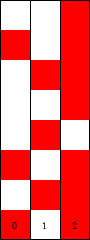
\includegraphics[width=.75\textwidth]{9/input.png}
		\caption{Input}
		\label{subfig:3neur_in}
	\end{subfigure}
	\hspace{1em}
	\begin{subfigure}{.3\textwidth}
		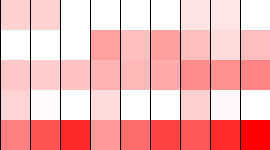
\includegraphics[width=\textwidth]{9/out0.png}
		\caption{Data after first transform}
	\end{subfigure}
	\hspace{1em}
	\begin{subfigure}{.3\textwidth}
		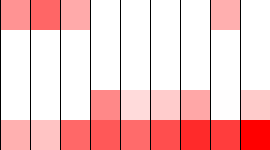
\includegraphics[width=\textwidth]{9/out1.png}
		\caption{Data after convolutional layer}
		\label{subfig:3neur_out1}
	\end{subfigure}
	\caption{Path of data through network, up to final transform}
	\label{fig:3neur_input}
\end{figure}

The last transformation of the network involves a matrix multiplication of the 
final layer weights\footnote{see appendix} with the data in 
\ref{subfig:3neur_out1}. This produces the adjacency matrix found in figure 
\ref{fig:3neur_pred}.

\begin{table}[h]
	\centering
	\adjacencyT{.02 & .03 & .01}{.99 & .01 & -.01}{1.0 & 1.0 & .02}
	\captionof{figure}{Model prediction for input data in 
	\figref{subfig:3neur_in}}
	\label{fig:3neur_pred}
\end{table}

\section{Applicability Beyond Training Data}
As described in \ref{subsec:hotswap}, the fact that our model is trained on data 
produced by only one generator is of little consequence; due to its structure, 
the only information it can learn is relational; i.e., per-neuron-pair. Consider 
the following examples, in which data was produced from several generator 
networks and fed into the model described in \ref{results_3neur}:


TODO: add examples of input and output data to 3.2.1 and 3.2.2.

\subsection{Inverted Network}
\begin{table}[h]
	\centering
	\begin{tikzpicture}[baseline=(current bounding box.center),->,>=stealth', 
	node distance=5em, semithick]
	\tikzstyle{every state}=[fill=none, draw=black, text=black]

		\node[state] (0) {0};
		\node[state] (1) [right of=0] {1};
		\node[state] (2) [below right of=0] {2};
	
		\path 	(2) edge node {} (1)
				(2) edge node {} (0)
				(1) edge node {} (0);
	\end{tikzpicture}
	\hspace{2em}
	\begin{tabular}{l|lll}
		  & 0 & 1 & 2\\
		\hline
		0 & 0 & 1 & 1\\
		1 & 0 & 0 & 1\\
		2 & 0 & 0 & 0
	\end{tabular}
	\captionof{figure}{Inverted version of \figref{fig:2simplex+adjacency}}
	\label{fig:2simplexVar1}
\end{table}
\noindent Despite being a complete inversion of the generator used to train the 
model in \ref{results_3neur}, reconstruction of this network is simple.

\begin{table}[h]
	\centering
	\begin{minipage}{.1\textwidth}
		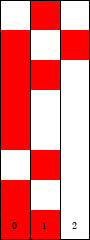
\includegraphics[width=\textwidth]{var1/input.png}
	\end{minipage}
	\hspace{2em}
	{\scalebox{2}{$\Rightarrow$}}
	\hspace{2em}
	\begin{tabular}{l|lll}
		  & 0 & 1 & 2\\
		\hline
		0 & .01 & 1.00 & 1.00\\
		1 & .01 & .02 & 1.00\\
		2 & 0 & .02 & .01
	\end{tabular}
\end{table}

\subsection{Cyclical Network}
\label{subsec:cyclical}
\begin{table}[h]
	\centering
	\begin{tikzpicture}[baseline=(current bounding box.center),->,>=stealth', 
	node distance=5em, semithick]
	\tikzstyle{every state}=[fill=none, draw=black, text=black]

		\node[state] (0) {0};
		\node[state] (1) [right of=0] {1};
		\node[state] (2) [below right of=0] {2};
	
		\path 	(2) edge node {} (1)
				(0) edge node {} (2)
				(1) edge node {} (0);
	\end{tikzpicture}
	\hspace{2em}
	\begin{tabular}{l|lll}
		  & 0 & 1 & 2\\
		\hline
		0 & 0 & 1 & 0\\
		1 & 0 & 0 & 1\\
		2 & 1 & 0 & 0
	\end{tabular}
	\captionof{figure}{Cyclical 3-neuron network}
	\label{fig:2simplexVar2}
\end{table}

\noindent For a cyclical network, the situation is not quite so simple. Due to 
the perpetual propagation of spikes through the generator, additional random 
spiking can cause the input data to become an impenetrable mess. Tempering the 
spike rate to 0.05 produces workable data, but the results are neither so clean 
nor
consistent as for terminating networks.  


